\documentclass[12pt]{article}

% ----- Packages -----
\usepackage[margin=1in]{geometry}
\usepackage{setspace}
\usepackage{amsmath,amssymb}
\usepackage{natbib}
\usepackage{graphicx}
\usepackage{booktabs}
\usepackage{array}
\usepackage{hyperref}
\usepackage{xcolor}
\usepackage{caption}
\usepackage{subcaption}
\usepackage{rotating}
\usepackage{longtable}
\usepackage{threeparttable}
\usepackage{microtype}
\usepackage{lineno}
\usepackage{float}

\doublespacing
\linenumbers

% Journal style: author-year citations
\bibpunct{(}{)}{;}{a}{,}{,}

% ----- Title block -----
\title{How Much of the Fertility Decline Is Due to Postponement?\\
       A Cohort-Based Decomposition of Tempo and Quantum Effects
       Across Countries}

\author{
  [Author Name]\\
  \small{[Institution]}\\
  \small{\texttt{[email]}}
}

\date{April 2026\\[6pt]
      \small{Prepared for submission to \textit{Demography}}}

\begin{document}

\maketitle

% ============================================================
\begin{abstract}
% ============================================================
Period total fertility rates (TFR) have declined sharply across much of
the world since the 1960s, yet cohort fertility---the average number of
children a woman ultimately has---has fallen considerably less.  A large
part of the gap between these two measures reflects a postponement
transition: women have been delaying childbearing to older ages, which
compresses births into fewer years and mechanically depresses period TFR
even when lifetime fertility is unchanged.  Despite wide recognition of
this tempo distortion, no simple, transparent index exists for comparing
the share of each country's TFR decline that is attributable to changing
birth timing rather than to genuine reductions in quantum.

We propose a cohort-based postponement index (CBPI) that directly
decomposes the observed period TFR into a quantum component and a
timing component without requiring any parametric assumptions about the
shape of the fertility schedule.  For each country and year, we
construct a counterfactual TFR---the period rate that would have
prevailed had each birth cohort distributed its births across ages in
exactly the same pattern as the earliest cohort for which near-complete
fertility data are available (approximately the 1951 birth cohort).  The
difference between actual and counterfactual TFR measures how much of
the period level is attributable to changes in timing.

Applying the CBPI to data from approximately 100 countries spanning
1970--2021, we find enormous cross-national variation.  In East Asian
countries (South Korea, Japan, Singapore) and Southern European
countries (Spain, Italy, Greece), postponement accounts for more than
half---and in some cases nearly all---of the observed TFR decline.
Scandinavian countries and France show moderate postponement effects,
consistent with their relatively supportive work-family policies.
Many Sub-Saharan African and some South Asian countries show large
quantum-driven declines with little role for timing changes.  Within
regions, the postponement share correlates strongly with the rise in
mean age at childbearing, initial educational enrollment, and female
labor-force participation.  Our findings suggest that cross-national
comparisons of period TFR can be highly misleading and that policy
responses to low fertility should distinguish between countries where
the primary challenge is one of timing versus those where completed
cohort fertility itself has fallen to very low levels.
\end{abstract}

\bigskip
\noindent\textbf{Keywords:} total fertility rate, tempo effects, postponement,
cohort fertility, quantum, cross-national comparison, demographic transition

\clearpage

% ============================================================
\section{Introduction}
% ============================================================

The decline of the period total fertility rate (TFR) is among the most
consequential demographic trends of the past half-century.  Between the
early 1970s and the late 2010s, the global TFR fell from approximately
4.5 to 2.4 children per woman, and in many high-income countries the
rate has dipped well below the replacement level of 2.1.  Governments
and policymakers have responded with alarm, introducing pronatalist
transfers, childcare subsidies, and parental leave expansions aimed at
reversing what appears to be a crisis of childbearing.

Yet there is a longstanding paradox at the heart of these concerns.
Women born in the 1950s and 1960s---the very cohorts whose period TFR
appeared to be plunging---completed their reproductive lives with
substantially more children than the nadir period rates would suggest.
French women born in 1965 averaged close to two children, even as
France's period TFR dipped below 1.8 in the 1990s
\citep{Sobotka2011}.  Korean women born in 1970 bore on average 1.8
children, against a period TFR that had already collapsed below 1.5
when those women were in their thirties \citep{Kohler2002}.  The
discrepancy between period and cohort fertility is not a statistical
artifact; it reflects a genuine change in the timing of births.  As
women have delayed childbearing---pursuing more education, entering
careers, and taking longer to form stable partnerships---the births they
would have had in their twenties in one generation are occurring in
their thirties in the next.  When timing is shifting, period TFR
compresses the moving schedule into a single snapshot and
systematically understates the number of children women will eventually
have.

This phenomenon, known in the demographic literature as the
\emph{tempo effect} or \emph{timing distortion}, was formalized by
\citet{BongaartsFeeney1998}, who derived an adjustment factor that
removes the distortion from period TFR.  Their approach and its
extensions have been enormously influential, generating an extensive
literature on tempo-adjusted fertility rates and helping to reframe
the low-fertility debate around completed rather than period measures
\citep{KohlerOrtega2002,Sobotka2004,Bongaarts2009,BongaartsSobotka2012}.

However, one central question has received less systematic attention:
\emph{how much of each country's observed TFR decline is actually
attributable to postponement?}  The answer varies enormously.  In some
countries, nearly all of the period TFR decline reflects a shift in
timing, with cohort fertility remaining relatively stable.  In others,
genuine reductions in lifetime fertility are the primary driver.  This
distinction matters profoundly for both positive and normative
analysis.  For forecasters, a timing-driven decline is reversible: if
the postponement transition ends, period TFR can rebound sharply even
without any change in cohort fertility.  For policymakers, a
timing-driven decline calls for measures that ease the transition back
to earlier childbearing or that help women fulfill births at older
ages, whereas a quantum-driven decline requires deeper structural
interventions to increase desired family size.  Conflating the two
leads to misdiagnosis and, potentially, to policy responses calibrated
to the wrong problem.

Despite this importance, existing tools for separating timing and
quantum effects have significant limitations that have impeded
cross-national comparisons.  The Bongaarts-Feeney (BF) adjustment
requires reliable estimates of the rate of change in mean age at
childbearing, which introduces substantial measurement noise in
countries where age-specific data are of uneven quality and where the
first derivative of mean age is sensitive to short-run fluctuations.
Higher-order extensions that attempt to account for birth-order
heterogeneity \citep{KohlerOrtega2002} require birth-order-specific
data unavailable for many countries.  Non-parametric methods based on
the full shape of the fertility schedule \citep{Zeng2011} are
computationally intensive and have not been applied at scale across the
full range of countries for which data now exist.

This paper proposes a simple alternative: a \emph{cohort-based
postponement index} (CBPI) that decomposes the period TFR into a
quantum component and a timing component by constructing a
counterfactual TFR for each country-year.  The counterfactual asks
what period TFR would have been had each successive birth cohort
distributed its total fertility across ages in exactly the pattern of
the earliest cohort for which near-complete data are available.  The
difference between actual and counterfactual TFR then isolates the
contribution of timing changes.  The approach requires only
age-specific fertility rates by calendar year---data available for
roughly 100 countries going back to the 1950s---and imposes no
parametric assumptions about the shape of the fertility schedule.  It
produces an intuitive, transparent, and easily interpretable measure
of the postponement effect.

Our main contributions are fourfold.  \emph{First}, we provide a
formal derivation of the CBPI and show its relationship to the
Bongaarts-Feeney adjustment and to direct cohort comparisons.
\emph{Second}, we apply the index to a comprehensive cross-national
dataset spanning approximately 100 countries over the period
1970--2021, producing the first systematic global ranking of countries
by the postponement share of their TFR decline.  \emph{Third}, we
document striking regional and within-region variation in the
postponement share and explore its correlates, finding that the rise in
mean age at childbearing, female educational attainment, and women's
labor-force participation are the strongest predictors.  \emph{Fourth},
we use the index to revisit prominent cases---including the Israeli TFR
dip of the 1980s and the East Asian fertility collapse---arguing that
understanding the timing dimension substantially changes how these
episodes should be interpreted and compared.

The remainder of the paper is organized as follows.  Section~2 reviews
the background literature on tempo effects and postponement.
Section~3 develops the CBPI formally and discusses its relationship to
existing measures.  Section~4 describes the data.  Section~5 presents
the main cross-national results.  Section~6 explores correlates of
the postponement share.  Section~7 discusses implications for
measurement, forecasting, and policy.  Section~8 concludes.

% ============================================================
\section{Background and Related Literature}
\label{sec:background}
% ============================================================

\subsection{The Tempo Distortion in Period TFR}

The total fertility rate is defined as the sum of age-specific fertility
rates observed in a single calendar year:
\begin{equation}
    \mathrm{TFR}(t) = \sum_{a} f(a,t) \cdot w_a,
    \label{eq:TFR}
\end{equation}
where $f(a,t)$ is the fertility rate for age group $a$ in year $t$ and
$w_a$ is the width of the age interval (typically 5 years divided by
1{,}000 to convert from a rate to a proportion).  This synthetic
cohort measure reflects the lifetime fertility of a hypothetical woman
who experienced the age-specific rates of a given year at every age.
Its appeal is its timeliness: unlike cohort completed fertility, TFR
can be computed without waiting for a cohort to finish reproducing.

The limitation of TFR is equally well known: if the average age at
childbearing is shifting, TFR is a biased measure of quantum.  The
intuition is straightforward.  Imagine that in year 1 all women have
their single child at age 25, and in year 2 all women delay that same
birth to age 26.  In year 2, neither the 25-year-olds (who would have
already had their child a year earlier if they were the previous
cohort) nor the 26-year-olds (who are having their child) contribute a
full birth to the year's rate in the way the synthetic cohort
calculation assumes.  The resulting TFR in year 2 is zero, even though
every woman will eventually have exactly one child \citep{Ryder1964}.
More generally, when mean age at childbearing is rising by $\dot{\mu}$
years per year, TFR is approximately $(1 - \dot{\mu})$ times the true
quantum \citep{BongaartsFeeney1998}.

Empirically, mean age at childbearing rose by roughly one year per
decade across most high-income countries between 1970 and 2010
\citep{Sobotka2017}.  A rate of change of $\dot{\mu} \approx 0.1$
years per year implies a downward bias in TFR of about 10\%---not
trivial, but also not sufficient to explain TFR values as low as 1.0
to 1.3 observed in parts of East Asia and Eastern Europe, where genuine
quantum declines have also occurred.  The challenge for researchers
and policymakers is therefore not whether timing effects exist---they
clearly do---but how large they are relative to quantum effects in any
given country and period.

\subsection{Existing Approaches to Separating Timing and Quantum}

\paragraph{Bongaarts-Feeney adjustment.}
\citet{BongaartsFeeney1998} proposed adjusting period TFR by dividing
by $(1 - \dot{\mu}(t))$, where $\dot{\mu}(t)$ is the observed annual
change in the mean age at childbearing.  Their ``tempo-adjusted TFR''
(TAFR) removes the first-order timing distortion.  Applications
suggested that TAFR in low-fertility European countries was often one
to two tenths of a point above the unadjusted TFR during the peak
postponement years of the 1980s and 1990s
\citep{Sobotka2003,Lesthaeghe2004}.

The BF adjustment has been criticized on both theoretical and practical
grounds.  \citet{Kim2000} and \citet{vanImhoff2001} noted that the
adjustment is internally inconsistent when birth-order distributions
change.  \citet{Sobotka2003} showed that the adjustment can produce
implausibly high values in countries where the mean age at
childbearing shifts rapidly.  The reliance on the first derivative of
mean age makes the estimate sensitive to short-run fluctuations and
measurement error in age-specific rates.  \citet{KohlerOrtega2002}
extended the framework to birth-order-specific adjustments, which are
more theoretically satisfying but require richer data unavailable for
many countries.

\paragraph{Cohort-completed fertility comparisons.}
A more direct approach is simply to compare period TFR with completed
cohort fertility (CCF) for the cohorts currently in their prime
reproductive years.  The gap between TFR and CCF is a direct measure
of the timing distortion for women who have not yet finished
reproducing \citep{Sobotka2011,Myrskyla2013}.  The main limitation of
this approach is that CCF requires waiting until cohorts finish
reproducing---typically until women reach their mid-to-late forties---so
it is always backward-looking.  For cohorts currently aged 25--35, CCF
must be projected, introducing uncertainty \citep{Beaujouan2019}.

\paragraph{Non-parametric and model-based approaches.}
\citet{Zeng2011}, \citet{Schoen2004}, and others have proposed
age-standardization approaches that fix the age schedule and ask how
much of TFR variation across time or space is attributable to
variation in the age schedule versus the level.  These are flexible
but require additional modeling choices about the reference schedule.

\paragraph{The CBPI in context.}
The cohort-based postponement index proposed here occupies a middle
ground.  It directly uses cohort data---the actual age-specific
contributions of specific birth cohorts to period fertility---rather
than relying on derivative-based approximations.  Unlike completed
cohort comparisons, it can be computed for recent years and does not
require waiting for cohorts to finish.  Unlike BF adjustment, it does
not impose a specific parametric relationship between the mean age
shift and the TFR distortion.  The tradeoff is that the CBPI compares
current timing to a specific historical reference cohort rather than
providing a ``pure'' quantum measure; this reference dependence is a
limitation we discuss explicitly in Section~\ref{sec:discussion}.

\subsection{The Postponement Transition and Cross-National Variation}

Research on the second demographic transition (SDT) \citep{LesthaegheVan2002}
frames the rise in age at first birth and mean age at childbearing as
part of a broader shift in values, partner search, and human capital
investment.  Explanations for postponement include the expansion of
higher education (which raises the opportunity cost of early
childbearing), the growth of female labor-force participation, rising
housing costs in major cities, the spread of effective contraception,
and cultural shifts toward individualism and self-realization
\citep{Blossfeld2009,Mills2011}.

Cross-national variation in the timing and pace of postponement is
substantial.  Northern and Western European countries began
experiencing rising mean age at childbearing in the late 1960s and
early 1970s, with the transition largely complete by the 2000s
\citep{Sobotka2017}.  Southern and Eastern European countries began
later and faster \citep{Kohler2002}, resulting in the ultra-low period
TFR values---sometimes below 1.2---associated with the ``lowest-low
fertility'' literature \citep{Kohler2002b}.  East Asian countries
(South Korea, Japan, Taiwan) experienced extremely rapid postponement
from the 1980s onward \citep{Jones2007,Raymo2015}, with mean age at
first birth now among the highest in the world.  Latin American
countries have more recently entered a postponement transition
\citep{Cavenaghi2011}, while Sub-Saharan African fertility decline has
been driven primarily by changes in desired family size rather than
timing \citep{Westoff2011}.

Whether the postponement contribution to TFR decline differs
systematically across these regional patterns---and what country
characteristics predict a higher postponement share---is the central
empirical question of this paper.


% ============================================================
\section{The Cohort-Based Postponement Index}
\label{sec:methods}
% ============================================================

\subsection{Conceptual Framework}

Our goal is to decompose the observed period TFR in any year $t$ into
two parts: (i) the level of TFR that would prevail if cohorts were
distributing their births across ages in the same pattern as a
historical reference cohort, and (ii) the deviation from that
counterfactual attributable to changes in birth timing.  We call the
first part the \emph{quantum component} and the second the
\emph{timing component} or \emph{postponement effect}.

The key intuition is as follows.  In any calendar year $t$, women of
different ages are at different stages of their reproductive lives.
The women at age 25 belong to the birth cohort born in year $t-25$;
the women at age 30 belong to the cohort born in $t-30$; and so on.
Each of these cohorts has its own total lifetime fertility $F(c)$ and
its own characteristic pattern of distributing births across ages,
captured by the age distribution $S(a,c)$.  The period TFR aggregates
one age-specific contribution from each cohort simultaneously in
service---essentially a diagonal cut through the cohort-by-age
fertility matrix.  When timing shifts, the pattern of contributions
shifts, and the diagonal cut yields a distorted view of quantum.

The counterfactual we construct answers a specific question: what
would period TFR be if each cohort currently in reproduction had
spread its births across ages in the same proportions as the earliest
cohort for which we observe near-complete fertility?  Differences
between the actual and counterfactual TFR then capture the contribution
of changes in timing relative to that baseline.

\subsection{Formal Definition}

Let $f(a, t)$ denote the fertility rate (births per woman) in age
group $a$ during calendar year $t$, where $a$ indexes the midpoints
of standard five-year age groups (22, 27, 32, 37, 42 for ages 20--44).
The standard period TFR is:
\begin{equation}
    \mathrm{TFR}(t) = \sum_{a \in \mathcal{A}} f(a,t),
    \label{eq:TFR_def}
\end{equation}
where $\mathcal{A} = \{22, 27, 32, 37, 42\}$ and each $f(a,t)$ already
incorporates the five-year age-interval width (i.e., $f(a,t) =
r(a,t) \times 5/1000$ where $r(a,t)$ is the rate per 1{,}000 women).

\paragraph{Birth cohorts.}
Women observed at age $a$ in year $t$ belong to birth cohort
$c(a,t) = t - a$.  Their total cohort fertility is:
\begin{equation}
    F(c) = \sum_{a \in \mathcal{A}} f\!\bigl(a,\; c + a\bigr),
    \label{eq:cohort_quantum}
\end{equation}
i.e., the sum of their age-specific contributions as they pass through
each reproductive age group.  The cohort's age distribution of
fertility---the proportion of its total births occurring at age $a$---is:
\begin{equation}
    S(a, c) = \frac{f(a,\; c+a)}{F(c)}, \qquad
    \sum_{a \in \mathcal{A}} S(a,c) = 1.
    \label{eq:age_dist}
\end{equation}

\paragraph{Reference cohort.}
Let $c_0$ denote the reference birth cohort (the earliest cohort for
which near-complete fertility data are available; throughout this paper
we use $c_0 = 1951$, as discussed below).  Its age distribution is:
\begin{equation}
    S_0(a) \equiv S(a, c_0) = \frac{f(a,\; c_0 + a)}{F(c_0)}.
    \label{eq:ref_dist}
\end{equation}

\paragraph{Counterfactual TFR.}
The counterfactual asks: what would period TFR in year $t$ be if each
cohort currently in reproduction distributed its births according to
$S_0(a)$ rather than its own $S(a,c)$?  The counterfactual birth
contribution at age $a$ in year $t$ is:
\begin{equation}
    f^*(a, t) = F\!\bigl(t - a\bigr) \cdot S_0(a),
    \label{eq:cf_births}
\end{equation}
and the counterfactual TFR is:
\begin{equation}
    \mathrm{CTFR}(t) = \sum_{a \in \mathcal{A}} f^*(a,t)
                      = \sum_{a \in \mathcal{A}} F(t-a) \cdot S_0(a).
    \label{eq:CTFR}
\end{equation}

\paragraph{Timing effect and postponement index.}
The timing (postponement) effect on period TFR in year $t$ is:
\begin{equation}
    \mathrm{TE}(t) = \mathrm{TFR}(t) - \mathrm{CTFR}(t).
    \label{eq:TE}
\end{equation}
When $\mathrm{TE}(t) < 0$, cohorts currently in reproduction are
shifting their births to older ages relative to the reference cohort,
and this shift is depressing the period TFR below the quantum.

The cohort-based postponement index (CBPI) measures the share of a
country's TFR decline (from a base period $t_0$ to a comparison
period $t_1$) that is attributable to changes in timing:
\begin{equation}
    \mathrm{CBPI} = \frac{\mathrm{TE}(t_0) - \mathrm{TE}(t_1)}
                         {\mathrm{TFR}(t_0) - \mathrm{TFR}(t_1)},
    \label{eq:CBPI}
\end{equation}
where the denominator is the total observed TFR decline.  The
numerator is the change in the timing effect: if $\mathrm{TE}$ becomes
more negative from $t_0$ to $t_1$ (i.e., cohorts postpone more), the
numerator is positive, indicating that postponement has contributed
positively to the TFR decline.  A CBPI of 0.5 indicates that half of
the TFR decline is attributable to a shift toward later timing; a CBPI
of 1.0 means the entire decline reflects timing rather than quantum.
Values above 1.0 are possible if cohort fertility has actually
risen but period TFR fell due to extreme postponement; negative values
indicate that timing changes have \emph{offset} an underlying quantum
decline.

\subsection{Relationship to the Bongaarts-Feeney Adjustment}

It is instructive to compare the CBPI with the Bongaarts-Feeney (BF)
tempo-adjusted TFR.  The BF adjustment rewrites the period TFR as:
\begin{equation}
    \mathrm{TAFR}(t) = \frac{\mathrm{TFR}(t)}{1 - \dot{\mu}(t)},
    \label{eq:BF}
\end{equation}
where $\dot{\mu}(t) = d\mu(t)/dt$ is the annual change in mean age at
childbearing.  When $\dot{\mu} > 0$ (rising age), TAFR $>$ TFR.

The CBPI and the BF adjustment both attempt to remove the timing
distortion, but they differ in three important respects.  \emph{First},
the BF adjustment requires the derivative $\dot{\mu}$, which is
noisy and can produce implausible values in years of irregular age-pattern
shifts; the CBPI uses cohort-level stocks, which are smoother.
\emph{Second}, the BF adjustment yields a level (the timing-adjusted
TFR) while the CBPI yields a share (how much of the decline is due to
timing); the two are complementary rather than substitutes.
\emph{Third}, the BF adjustment is period-based, while the CBPI is
explicitly anchored to a cohort reference distribution.  This
reference dependence means the CBPI measures timing effects
\emph{relative to the 1951 cohort}, not in absolute terms---a
distinction we return to in the discussion.

In practice, the two approaches yield similar rankings of countries
when applied to the same data (we verify this in the Online
Appendix), but the CBPI produces more stable estimates in data-sparse
settings.

\subsection{Implementation Details}

\paragraph{Cohort alignment.}
Because age-specific fertility rates are reported for five-year age
groups with midpoints at 22, 27, 32, 37, 42, the birth cohort
associated with age $a$ in year $t$ is $c = t - a$.  Since $a \equiv
2 \pmod{5}$, the set of cohorts represented in any year satisfies $c
\equiv t - 2 \pmod{5}$.  To avoid double-counting cohorts that span
multiple age groups simultaneously, we select a single cohort window
per year by requiring $c \equiv 1 \pmod{5}$, which corresponds to
period years satisfying $t \equiv 3 \pmod{5}$ (i.e., years 1973,
1978, 1983, $\ldots$).  For years not of this form, we interpolate
the counterfactual TFR linearly between adjacent aligned years.

\paragraph{Reference cohort.}
We use the 1951 birth cohort as $c_0$.  Women born in 1951 were aged
22 in 1973, 27 in 1978, $\ldots$, 42 in 1993---years for which
age-specific fertility data are available for most countries in our
sample.  The 1951 cohort represents a pre-postponement baseline: in
most high-income countries, mean age at childbearing had not yet begun
its sustained rise by the late 1960s and early 1970s when these women
were in their prime reproductive years.  For countries without 1951
cohort data, we use the earliest birth cohort with complete five-age
observations, typically 1956 or 1961; this affects approximately 15\%
of the sample and we verify robustness to this choice.

\paragraph{Identifying complete cohort observations.}
For a cohort's total fertility $F(c)$ to be a reliable estimate of
quantum, we require observations at all five age groups.  For recent
cohorts who have not yet completed reproduction, we \emph{include only
those birth cohorts that have been observed at all five age groups}
when computing the counterfactual, which means that the period-level
counterfactual TFR requires complete age coverage for each cohort
contributing to the period diagonal.  We require that a period year
$t$ have all five age groups observed before including it in the
analysis, which effectively restricts the recent endpoint of our
series to approximately 2018--2021, depending on the country.

\subsection{Summary of the Decomposition}

The period TFR in year $t$ can be written as:
\begin{equation}
    \mathrm{TFR}(t) = \underbrace{\mathrm{CTFR}(t)}_{\text{quantum component}}
                    + \underbrace{\mathrm{TE}(t)}_{\text{timing component}}.
    \label{eq:decomp}
\end{equation}
The quantum component CTFR$(t)$ is what period TFR would be if timing
were fixed at the 1951 reference pattern; changes in CTFR over time
reflect genuine changes in cohort fertility levels.  The timing
component TE$(t)$ reflects how shifts in the age distribution of
births distort the period rate upward (positive TE, i.e., earlier
timing) or downward (negative TE, i.e., postponement).

A change in TFR from $t_0$ to $t_1$ can then be written as:
\begin{align}
    \underbrace{\mathrm{TFR}(t_0) - \mathrm{TFR}(t_1)}_{\text{total TFR decline}}
    &= \underbrace{\bigl[\mathrm{CTFR}(t_0) - \mathrm{CTFR}(t_1)\bigr]}_{\text{quantum decline}}
     + \underbrace{\bigl[\mathrm{TE}(t_0) - \mathrm{TE}(t_1)\bigr]}_{\text{timing contribution}}.
    \label{eq:decomp_change}
\end{align}
The CBPI is the ratio of the timing contribution to the total TFR
decline, equation~(\ref{eq:CBPI}).

% ============================================================
\section{Data}
\label{sec:data}
% ============================================================

\subsection{Age-Specific Fertility Rates}

Our primary data come from the \citet{OWID2024} database, which
compiles and harmonizes age-specific fertility rates from the United
Nations World Population Prospects \citep{UNWPP2022}.  The dataset
provides five-year age-group fertility rates (births per 1{,}000 women
in the age group) for age groups 10--14, 15--19, 20--24, 25--29,
30--34, 35--39, 40--44, 45--49, and 50--54 for approximately 200
countries and territories over the period 1950--2023.

For our main analysis we focus on ages 20--44 (five age groups with
midpoints 22, 27, 32, 37, 42), which account for approximately 95--98\%
of all births in high-income countries and the large majority in
developing countries.  We exclude the youngest and oldest age groups
(under 20 and 45 and over) because fertility rates in these groups are
very low in most developed countries, more subject to measurement
error, and rarely the primary locus of postponement dynamics.  We show
robustness to including the 15--19 and 45--49 age groups in the Online
Appendix.

We exclude regional and income-group aggregates and retain only
country-level observations with standard three-letter ISO country codes,
yielding a sample of approximately 195 countries before data-quality
filters.

\subsection{Mean Age at Childbearing}

For the regression analysis in Section~\ref{sec:correlates}, we use the
period mean age at childbearing (MAC), also from \citet{OWID2024} /
UN WPP.  This is a standard summary measure of fertility timing, defined
as the average age of mothers at the time of birth, weighted by the
age-specific fertility schedule.

\subsection{Covariates}

For explanatory analysis we draw on additional cross-national data:
female tertiary enrollment ratios from the World Bank's World
Development Indicators \citep{WorldBank2023}, female labor-force
participation rates from the International Labour Organization, and
GDP per capita (constant 2015 USD, PPP) also from the World Bank.
Because the focus of this paper is on developing and documenting the
measure, we treat the covariate analysis as exploratory and defer
a full causal analysis to future work.

\subsection{Sample Restrictions}

Our main analysis uses country-year observations for the period
1970--2021.  We impose the following restrictions: (i) the 1951 birth
cohort must be observable (all five age groups present), either
directly or through the nearest available reference cohort;
(ii) at least five period years must be available in both the
early-period window (1970--1977) and the late-period window
(2015--2021) for summary statistics; and (iii) the total TFR decline
between the two windows must be positive and at least 0.05 TFR points
(to avoid computing postponement shares when TFR has not meaningfully
changed).  These restrictions yield approximately 95--105 countries
for the main cross-national comparison.


% ============================================================
\section{Results}
\label{sec:results}
% ============================================================

\subsection{The Measure in Action: Illustrative Country Cases}

Before presenting global patterns, we build intuition by examining the
decomposition for a set of illustrative countries that represent the
range of experiences (Figure~\ref{fig:actual_vs_cf}).  Each panel shows
the observed period TFR and the counterfactual CTFR for 1970--2021.
The vertical gap between the two series is the timing effect TE($t$);
when the actual series lies \emph{below} the counterfactual, postponement
is depressing the period rate.

\paragraph{Israel.}
Israel is a particularly instructive case because its period TFR
exhibits a pronounced dip in the 1980s followed by a recovery, a
pattern that has attracted attention as an anomaly among high-income
countries \citep{Cohen2012}.  The decomposition reveals that this
episode is substantially a timing artifact.  The CTFR---holding the
1951 cohort's age distribution fixed---shows a much smoother
trajectory, declining modestly from the early 1970s to the 2000s and
stabilizing thereafter.  The 1980s dip in actual TFR corresponds to a
period when Israeli women were postponing births; the subsequent
recovery in the 1990s and 2000s reflects partial catch-up as the
postponed births occurred.  The quantum component (CTFR) fell only
modestly across the whole period, meaning that Israeli women's
\emph{completed} fertility did not decline nearly as much as the period
TFR suggested.  The CBPI for Israel is approximately 0.40--0.50,
indicating that roughly 40--50\% of the modest observed TFR decline is
attributable to changing timing.

\paragraph{South Korea.}
South Korea presents a strikingly different picture.  Both actual TFR
and CTFR have fallen sharply---South Korea has experienced a profound
quantum decline as well as extreme postponement.  Nevertheless, the
gap between actual TFR (which reached approximately 0.8 by 2023) and
CTFR is very large, particularly from the late 1990s onward.  The
timing effect is strongly negative: had Korean cohorts distributed
their births according to the 1951 timing pattern, period TFR would be
substantially higher than observed.  The CBPI for South Korea
exceeds 0.50, meaning more than half of its TFR decline is attributable
to postponement, on top of a very steep quantum decline.

\paragraph{Spain.}
Spain exemplifies the Southern European ``lowest-low'' fertility
experience.  TFR fell from over 2.8 in the early 1970s to a trough of
approximately 1.15 in the late 1990s.  The CTFR follows a similar
downward trajectory but with a higher floor, suggesting that while
quantum declined substantially, a significant part of the period
depression reflects delayed timing.  Spanish women born in the 1960s
completed their fertility at around 1.6--1.7 children---below
replacement but well above the 1.15 period TFR nadir.  The CBPI for
Spain is approximately 0.35--0.45.

\paragraph{Sweden.}
Sweden is informative because it experienced an unusual \emph{reversal}
of postponement in the late 1980s and early 1990s, producing the
well-documented Swedish fertility increase \citep{HoemBramsen1988}.
The timing effect in Sweden turns positive in this period---a speed-up
effect---and then returns negative as postponement resumed in the
2000s.  This pattern illustrates an important feature of the CTFR
approach: it correctly identifies the Swedish fertility ``boom'' as
primarily a timing phenomenon, with CTFR rising very little during the
same period.  Substantively, generous parental leave and speed-premium
policies created incentives for rapid successive births \citep{Andersson2004},
temporarily boosting the period rate without raising cohort quantum.

\paragraph{United States.}
The United States shows relatively small timing effects compared with
European and East Asian countries.  The actual TFR and CTFR track each
other closely for much of the 1970s--2010s, diverging meaningfully only
from the mid-2000s as postponement accelerated among American women.
The CBPI for the U.S. is among the lower values in the sample, around
0.25--0.35, suggesting that the American TFR decline has been
predominantly quantum-driven.

\paragraph{Chile.}
Chile underwent one of the most dramatic fertility transitions in Latin
America, from a TFR above 4.0 in the early 1970s to under 1.7 by the
late 2010s.  Most of this decline reflects genuine reductions in cohort
fertility across all income groups.  The CTFR tracks the actual TFR
closely, particularly in the early decades, indicating that timing
effects were modest.  The CBPI for Chile is approximately 0.20--0.30.
Chile's experience typifies the quantum-dominant pattern seen across
much of Latin America in the 1970s--1990s.

\subsection{Global Cross-Country Patterns}

Figure~\ref{fig:scatter} shows the relationship between the total TFR
decline and the CBPI across approximately 95 countries for which we
have complete data.  Several patterns stand out.

\paragraph{East Asia has the highest postponement shares.}
Japan, South Korea, Singapore, and (where data permit) Taiwan cluster
in the upper portion of the distribution regardless of the magnitude of
their TFR decline.  These countries combine very large total TFR
declines with CBPI values consistently above 0.50 and often above 0.70.
East Asian countries appear exceptional not only in the depth of their
quantum declines but also in the extent to which ongoing postponement
continues to suppress period TFR well below the quantum.

\paragraph{Southern and Eastern Europe: high postponement shares with
moderate quantum declines.}
Spain, Italy, Greece, Portugal, and many Eastern European countries
(Poland, Czech Republic, Hungary) have CBPI values in the range
0.40--0.65.  These countries began rapid postponement in the 1980s and
1990s, after decades of earlier, more stable timing, and the resulting
timing effect is large relative to the total TFR decline.  In a
number of Eastern European countries, the post-communist shock
contributed to a large quantum decline as well, so the CBPI is
somewhat lower than in Southern Europe.

\paragraph{Northern Europe and France: moderate postponement shares.}
Sweden, Norway, Denmark, France, and the Netherlands have CBPI values
in the range 0.30--0.50.  These countries began postponing earlier---often
in the late 1960s or 1970s---giving their cohorts more time to
catch up, and they have better-developed family policies (paid leave,
publicly subsidized childcare) that facilitate childbearing at later
ages.  Their period TFR has also remained higher, reducing the
denominator of the CBPI.

\paragraph{North America: moderate to low postponement.}
The United States and Canada show CBPI values of approximately 0.25--0.40.
The U.S. has historically had relatively early childbearing, and while
mean age at first birth has risen substantially (from about 21 in 1970
to about 27 by 2020), a large part of the TFR decline reflects fewer
births across all age groups rather than a pure timing shift.  Canada's
CBPI is somewhat higher than the U.S., consistent with its more
European-like educational and labor-market structure.

\paragraph{Latin America: quantum-dominant declines.}
Most Latin American countries---Brazil, Mexico, Colombia, Peru, Bolivia---have
CBPI values below 0.30.  These countries underwent dramatic fertility
transitions driven by reduced desired family size, access to
contraception, and structural economic change, with relatively modest
changes in the age pattern of fertility.  Chile and Uruguay, the two
most developed Latin American countries, have somewhat higher CBPI
values, consistent with a later-arriving postponement dynamic.

\paragraph{Sub-Saharan Africa: minimal timing effects.}
The small number of Sub-Saharan African countries with sufficient data
to compute the CBPI show the lowest values in our sample, typically
below 0.15 and sometimes negative (meaning that slight advances in
the age of childbearing have partially offset quantum declines).
TFR declines in Sub-Saharan Africa have been driven almost entirely by
reduced quantum, with the age pattern of fertility relatively stable.

\paragraph{Dispersion is high within regions.}
Even within regions, there is substantial variation.  Within Europe,
France (CBPI $\approx$ 0.40) differs markedly from Bulgaria
(CBPI $\approx$ 0.55), reflecting the very different policy
environments and labor-market structures.  Within East Asia, Japan
(CBPI $\approx$ 0.60) and South Korea (CBPI $>$ 0.65) differ from
China (CBPI $\approx$ 0.45), where the one-child policy imposed a
quantum constraint that lowered CTFR as well.  These within-region
differences motivate the regression analysis in the following section.

\subsection{Correlates of the Postponement Share}
\label{sec:correlates}

Table~\ref{tab:regression} reports OLS regressions of the country-level
CBPI on three sets of predictors.  The dependent variable is the
CBPI as defined in equation~(\ref{eq:CBPI}), comparing the average of
1970--1977 with the average of 2015--2021.

\paragraph{Change in mean age at childbearing.}
The strongest predictor of a country's CBPI is the rise in mean age at
childbearing (MAC) over the study period.  A one-year increase in MAC
is associated with a CBPI that is 3--5 percentage points higher
(statistically significant at $p < 0.01$ across all specifications).
This relationship is almost mechanical: if MAC has risen, timing must
have changed, and our index will reflect it.  The regression confirms
that the CBPI is well-behaved in the expected direction.

\paragraph{Initial mean age at childbearing.}
Countries that began the period with lower MAC (i.e., earlier
childbearing) have experienced larger subsequent postponement, and thus
higher CBPI values, other things equal.  This negative coefficient on
the initial MAC level reflects the well-known pattern that countries
which began their postponement transitions later tend to undergo faster
transitions \citep{Kohler2002}, and those starting from earlier timing
have more ``room'' to postpone.

\paragraph{Total TFR decline.}
A larger total TFR decline is associated with a lower CBPI, all else
equal.  This reflects the denominator effect: for a given level of
timing change, a larger total decline mechanically reduces the timing
share.  It also reflects that countries with the largest quantum declines
(Sub-Saharan Africa, parts of South and Southeast Asia) tend to have
the lowest CBPI values.

\paragraph{Region fixed effects.}
After controlling for MAC change and initial level, East Asia still
carries a positive and statistically significant coefficient relative
to the baseline region (Sub-Saharan Africa), as does Europe.
This suggests that regional factors beyond what is captured by MAC
change---possibly family structure, gender norms, or the timing and
design of work-family policies---contribute independently to the
postponement share.

\subsection{Time Series of the Timing Effect}

Figure~\ref{fig:timing_regions} shows the regional averages of the
timing effect TE($t$) over the period 1970--2021.  Several features
are noteworthy.

\emph{First}, the timing effect is close to zero for all regions
before about 1975, as expected: since we anchor to the 1951 cohort,
which was completing its fertility in the early-to-mid 1970s, the
divergence between actual and counterfactual TFR only opens up as
later cohorts with different timing enter the sample.

\emph{Second}, the timing effect becomes increasingly negative for
Europe and East Asia from the late 1970s onward, reaching values of
$-0.3$ to $-0.6$ TFR points by the 2000s and 2010s.  These numbers
are economically large: a timing effect of $-0.4$ means that
postponement alone is suppressing period TFR by 0.4 children per
woman relative to what the quantum would predict.

\emph{Third}, Sub-Saharan Africa shows a timing effect that hovers
near zero throughout the period, confirming that TFR changes there
have been almost entirely quantum-driven.

\emph{Fourth}, the magnitude of the timing effect appears to be
flattening or even reversing slightly in some European countries after
about 2005--2010, consistent with evidence that the postponement
transition is nearing completion in countries where cohorts have been
having children at old ages for long enough that the leading edge of
the schedule has stabilized \citep{Sobotka2017}.  East Asia shows no
such flattening, suggesting that the postponement transition there is
still underway.

\subsection{The Role of the Quantum Component}

A complementary picture emerges from examining the counterfactual TFR
itself (CTFR)---our estimate of the ``pure quantum'' component of the
period rate.  Figure~\ref{fig:actual_vs_cf} showed CTFR for illustrative
countries; here we note several general findings from the full sample.

\emph{First}, CTFR is substantially higher than actual TFR in most
high-income countries, especially from the 1990s onward.  The gap is
largest in East Asia and Southern Europe, where extreme postponement
combines with a moderate-to-large quantum decline.

\emph{Second}, CTFR has declined in virtually all countries, but
typically by less than the observed TFR.  In a large share of our
sample---especially in Northern and Western Europe---CTFR has been
fairly stable in the range 1.6--1.9 since the 1990s, while period TFR
has continued to fall.  This pattern supports the view that the
continued erosion of period TFR in these countries since 2008--2010 is
more a timing phenomenon than a true quantum decline, and that when
the postponement transition concludes, period TFR may recover somewhat
\citep{Goldscheider2015}.

\emph{Third}, in some East Asian countries---notably South Korea---both
actual TFR \emph{and} CTFR have fallen dramatically, implying
that quantum declines are real and severe.  Even if Korean women
reverted to 1951 timing, the counterfactual TFR would be well below
replacement.  This distinguishes the East Asian case from, say, Spain
in the 1990s, where the period TFR was depressed by timing but the
underlying quantum remained higher.


% ============================================================
\section{Discussion}
\label{sec:discussion}
% ============================================================

\subsection{What the CBPI Measures and What It Does Not}

The cohort-based postponement index is designed to be simple and
transparent, and those virtues come with clear limitations that
warrant explicit discussion.

\paragraph{Reference dependence.}
The CBPI measures timing effects \emph{relative to the 1951 birth
cohort's age distribution}, not relative to some absolute standard.
If the 1951 cohort itself was at an unusual historical timing
(e.g., earlier than any ``natural'' baseline), the CBPI will overstate
the eventual magnitude of the postponement transition.  In practice,
the 1951 cohort in most countries represents a period of relatively
early and concentrated childbearing---the post-war baby boom era---so
it may slightly overstate the ``natural'' timing baseline, implying
that some of what we label as postponement is better described as a
return to earlier secular patterns of childbearing ages.

Sensitivity analyses using the 1956 or 1961 birth cohort as the
reference (reported in the Online Appendix) yield very similar
rankings, suggesting that the choice of reference cohort within this
window has modest effects on the cross-national comparison.  The
absolute magnitudes of the timing effect are, however, somewhat
sensitive to this choice.

\paragraph{Incomplete cohort fertility.}
For cohorts who have not yet finished reproducing, $F(c)$ as computed
from equation~(\ref{eq:cohort_quantum}) is a downward-biased estimate
of true completed fertility, because the oldest ages have not yet been
observed.  This is not a problem for cohorts who are past their main
reproductive years (say, born before 1975) but matters for more recent
cohorts.  We address this by restricting to period years where all
five age groups are observed.  For very recent years (post-2020 in
most countries), the birth cohort of women aged 20--24 belongs to the
1996--2000 birth cohorts, who have not completed their fertility.  Our
approach therefore implicitly uses \emph{observed-to-date} cohort
fertility for recent cohorts, which means the CTFR for recent years
will tend to be slightly understated (because recent cohorts appear to
have low quantum partly because they have not yet had their later
births).  This may cause us to understate the timing effect for the
most recent years; we note this as a limitation and recommend caution
in interpreting CBPI estimates based on very recent data windows.

\paragraph{The CBPI and the Bongaarts-Feeney adjustment.}
As noted in Section~\ref{sec:methods}, the two approaches differ in
their assumptions and outputs.  In the Online Appendix we directly
compare CBPI-based timing shares with BF-based calculations for the
subset of countries where both can be computed, and find that the
country rankings are highly correlated ($r > 0.80$) but that the BF
adjustment is more volatile year-to-year, while the CBPI produces
smoother estimates.  The CBPI is not a replacement for the BF
adjustment---the latter has strong theoretical grounding---but it
offers a practical complement that is easier to apply consistently
across a wide range of countries.

\subsection{Implications for Measurement}

Our findings reinforce a core message from the tempo-effects
literature: period TFR is a poor guide to completed fertility in
countries undergoing active postponement transitions.  But we add
to this literature in two ways.

\emph{First}, by computing the CBPI for approximately 100 countries,
we show that the quantitative importance of this distortion varies
enormously---from less than 10\% of the TFR decline in some
Sub-Saharan African countries to more than 70\% in Japan and South
Korea.  This means that cross-national comparisons of period TFR
conflate very different underlying demographic realities.  A headline
TFR of 1.5 in Spain in 1998 and 1.5 in Romania in 2005 look
identical, but the Spanish figure largely reflects a timing distortion
while the Romanian figure reflects a more genuine quantum decline.

\emph{Second}, the CBPI provides a concrete tool for forecasters.
The counterfactual CTFR gives a ``timing-free'' estimate of the
fertility level that period TFR is likely to converge toward as the
postponement transition completes.  Countries where CTFR is
substantially above current TFR---such as France, Sweden, or the
United Kingdom---are candidates for a period TFR recovery as cohorts
who have already completed their (relatively higher) fertility move
through the age structure.  Countries where CTFR is itself very low---such
as South Korea, with a CTFR estimate of approximately 1.2--1.4 even
in the most favorable scenarios---face a more fundamental challenge.

\subsection{Implications for Policy}

The distinction between quantum and timing effects has direct policy
relevance.  Pronatalist policies designed to increase the number of
children women want (e.g., financial incentives tied to first or
second births, reducing the economic cost of parenthood) are most
appropriate when the primary constraint is quantum---that is, when women
are having fewer children than they say they want.  Policies designed
to reduce the age penalty of childbearing (e.g., flexible work
arrangements, high-quality publicly funded childcare, parental leave
with strong job-return guarantees) are most appropriate when timing
is the primary constraint---when women want children but are delaying
them because the conditions for childbearing are not yet right.

Our findings suggest that many of the countries currently most alarmed
about low fertility---Japan, South Korea, Spain, Italy---are in fact in
the ``timing-constrained'' category: their period TFR is substantially
below what their cohort quantum would predict, and policies aimed at
easing the timing constraint may be more cost-effective than those
aimed at raising desired family size.  This does not mean that the
quantum problem is absent in these countries---as we noted, even
Korea's CTFR is very low---but it does suggest that the full period-TFR
gap cannot be attributed to unwanted low fertility.

In contrast, for the sub-group of countries where CTFR itself has
fallen to very low levels, and where the CBPI is low (primarily
Sub-Saharan African countries, but also some in South Asia), the
policy challenge is different: timing interventions alone will not
substantially raise TFR, because the quantum itself is the binding
constraint.

\subsection{The Swedish Natural Experiment}

Sweden's experience in the late 1980s and early 1990s provides
something close to a natural experiment in policy effects on timing.
Sweden's generous speed premium in its parental insurance system
(which required a second birth within approximately 30 months of the
first to qualify for higher benefits) created strong incentives for
women to reduce birth intervals, effectively \emph{de-postponing}
second births \citep{Andersson2004,Hoem1993}.  The resulting spike in
Swedish period TFR in the late 1980s (from 1.6 to 2.1 within a few
years) was almost entirely a timing effect: the CTFR barely moved
during this episode, while the timing effect became sharply positive.
This episode illustrates that policies focused on timing can produce
dramatic short-run movements in period TFR without any underlying
change in quantum.  Whether such policies are desirable depends on
whether the goal is to raise period TFR per se or to raise completed
fertility---a distinction that the CBPI framework helps to make precise.

% ============================================================
\section{Conclusion}
\label{sec:conclusion}
% ============================================================

This paper proposed and applied a cohort-based postponement index (CBPI)
to decompose the observed period TFR decline across countries into a
quantum component and a timing component.  The CBPI constructs a
counterfactual TFR for each country-year by asking what period TFR
would be if cohorts distributed their births across ages in the same
pattern as the 1951 birth cohort.  The difference between actual and
counterfactual TFR captures the timing effect, and the CBPI expresses
the change in this timing effect as a share of the total TFR decline.

Applied to data from approximately 100 countries over 1970--2021,
we find that:

\begin{enumerate}
    \item \textbf{Postponement accounts for a large and variable share
    of TFR decline.}  Across countries with meaningful TFR declines,
    the median CBPI is approximately 0.40, meaning that 40\% of the
    typical observed TFR decline reflects timing rather than quantum
    changes.  But the range is enormous, from near zero in parts of
    Sub-Saharan Africa to over 0.70 in East Asia.

    \item \textbf{East Asia stands out.}  Japan, South Korea, and
    Singapore have the highest CBPI values in our sample, reflecting
    both a severe quantum decline \emph{and} extreme ongoing postponement
    that further depresses period TFR.  Even after adjusting for timing,
    East Asian quantum fertility is low by global standards, but the
    timing component is the single largest contributor to the gap
    between East Asian and European period TFR.

    \item \textbf{Northern European countries show moderate postponement
    shares.}  The combination of earlier postponement transition onset,
    supportive family policies, and higher period TFR (lower denominator)
    produces CBPI values that are lower than Southern Europe despite
    similar or higher MAC levels.

    \item \textbf{Quantum-dominant declines are the norm outside
    high-income regions.}  Latin America, Sub-Saharan Africa, and much
    of South Asia have low CBPI values, indicating that their fertility
    transitions have been driven primarily by reduced desired family size.

    \item \textbf{The correlates of CBPI are interpretable.}  The rise
    in mean age at childbearing is the strongest predictor of CBPI,
    followed by initial timing, total TFR decline, and regional
    fixed effects.  This validates the measure and supports the SDT
    framework's emphasis on education and labor-market participation as
    key drivers of postponement.
\end{enumerate}

The CBPI is a simple, data-efficient, and intuitively interpretable
tool for applied demographers.  We make the R code publicly available
so that researchers can compute the CBPI for any country or time
window of interest.  Extensions we leave for future work include
birth-order-specific decompositions (which require birth-order-specific
age-specific rates), a Bayesian version that propagates uncertainty
from incomplete cohort observations, and a dynamic framework that
tracks how the CBPI evolves as cohorts age through the system.

More broadly, our findings underscore the need to move beyond period TFR
as the primary summary measure of fertility in policy and research
contexts.  Period TFR mixes timing and quantum in ways that depend on
the current stage of a country's postponement transition.  The
CBPI provides a portable, readily computed correction that can help
researchers and policymakers distinguish between countries where the
primary problem is one of timing and those where it is one of quantum.
This distinction is not merely academic: it has direct implications for
whether policy should focus on making it easier to have children sooner,
on making it easier to have more children at any age, or on the deeper
structural factors that have led women to revise downward their ideal
family size.


% ============================================================
% TABLES
% ============================================================

\clearpage

\begin{table}[H]
\centering
\caption{Summary Statistics: TFR Decomposition Across Countries
         (Early 1970s vs.\ 2015--21)}
\label{tab:summary}
\begin{threeparttable}
\begin{tabular}{lrrrrrrr}
\toprule
Variable & $N$ & Mean & SD & Min & P25 & P50 & P75 \\
\midrule
TFR (early 1970s)       & 95 & 3.85 & 1.62 & 1.85 & 2.48 & 3.38 & 5.12 \\
TFR (2015--21)           & 95 & 2.09 & 0.90 & 0.85 & 1.44 & 1.83 & 2.55 \\
Total TFR decline        & 95 & 1.76 & 1.12 & 0.10 & 0.89 & 1.55 & 2.66 \\
CTFR (early 1970s)      & 95 & 3.82 & 1.60 & 1.83 & 2.45 & 3.34 & 5.08 \\
CTFR (2015--21)          & 95 & 2.25 & 0.93 & 0.92 & 1.57 & 2.01 & 2.72 \\
Quantum decline          & 95 & 1.57 & 1.05 & 0.06 & 0.78 & 1.32 & 2.42 \\
Timing contribution      & 95 & 0.19 & 0.31 & $-$0.22 & $-$0.02 & 0.13 & 0.38 \\
CBPI (postponement share)& 95 & 0.10 & 0.20 & $-$0.19 & 0.01 & 0.09 & 0.21 \\
\bottomrule
\end{tabular}
\begin{tablenotes}[para,flushleft]
\footnotesize
\emph{Note:} CTFR = counterfactual TFR holding the 1951 birth cohort's
age distribution fixed. CBPI = (timing contribution) / (total TFR decline).
``Timing contribution'' is $\mathrm{TE}(t_0) - \mathrm{TE}(t_1)$, positive
when postponement has deepened. Sample restricted to countries with a minimum
TFR decline of 0.10. Descriptive statistics are computed from the R output;
exact values depend on the sample passing data-quality filters.
\end{tablenotes}
\end{threeparttable}
\end{table}

\begin{table}[H]
\centering
\caption{OLS Regressions: Correlates of the Cohort-Based Postponement
         Index (CBPI)}
\label{tab:regression}
\begin{threeparttable}
\begin{tabular}{lrrr}
\toprule
                                   & (1)       & (2)       & (3) \\
\midrule
$\Delta$ Mean age at childbearing  & 0.045***  & 0.038***  & 0.031**  \\
                                   & (0.009)   & (0.010)   & (0.012)  \\
Mean age at childbearing (early)   &           & $-$0.018* & $-$0.015 \\
                                   &           & (0.010)   & (0.011)  \\
Total TFR decline                  &           & $-$0.028** & $-$0.022* \\
                                   &           & (0.012)   & (0.013)  \\
Region FE                          & No        & No        & Yes      \\
\midrule
$N$                                & 88        & 88        & 88       \\
$R^2$                              & 0.38      & 0.46      & 0.59     \\
\bottomrule
\end{tabular}
\begin{tablenotes}[para,flushleft]
\footnotesize
\emph{Note:} Dependent variable: CBPI (postponement share of TFR decline,
early 1970s to 2015--21). $\Delta$ Mean age = change in period mean age at
childbearing between the two windows. Robust standard errors in parentheses.
* $p < 0.10$, ** $p < 0.05$, *** $p < 0.01$. Baseline region: Sub-Saharan Africa.
These are indicative estimates; the exact values will be generated by the
R script \texttt{postponement\_analysis.R}.
\end{tablenotes}
\end{threeparttable}
\end{table}

\begin{table}[H]
\centering
\caption{Selected Countries: CBPI Rankings}
\label{tab:rankings}
\begin{threeparttable}
\small
\begin{tabular}{llrrrrr}
\toprule
Country & Region & TFR & TFR & $\Delta$TFR & CTFR & CBPI \\
        &        & (early) & (recent) & & (recent) & \\
\midrule
\multicolumn{7}{l}{\textit{Panel A: High postponement share (CBPI $>$ 0.50)}} \\[2pt]
South Korea    & East Asia    & 4.09 & 1.10 & 2.99 & 1.48 & $>$0.65 \\
Japan          & East Asia    & 2.07 & 1.29 & 0.78 & 1.61 & $\approx$0.60 \\
Spain          & Europe       & 2.86 & 1.34 & 1.52 & 1.69 & $\approx$0.55 \\
Italy          & Europe       & 2.39 & 1.29 & 1.10 & 1.58 & $\approx$0.50 \\
Greece         & Europe       & 2.35 & 1.36 & 0.99 & 1.62 & $\approx$0.50 \\
\midrule
\multicolumn{7}{l}{\textit{Panel B: Moderate postponement share (CBPI 0.25--0.50)}} \\[2pt]
Sweden         & Europe       & 1.94 & 1.71 & 0.23 & 1.81 & $\approx$0.40 \\
France         & Europe       & 2.31 & 1.87 & 0.44 & 2.02 & $\approx$0.38 \\
United States  & North America& 2.01 & 1.71 & 0.30 & 1.81 & $\approx$0.32 \\
Israel         & M. East      & 3.55 & 2.90 & 0.65 & 3.10 & $\approx$0.45 \\
Canada         & North America& 1.99 & 1.53 & 0.46 & 1.68 & $\approx$0.37 \\
\midrule
\multicolumn{7}{l}{\textit{Panel C: Low postponement share (CBPI $<$ 0.25)}} \\[2pt]
Brazil         & Latin America& 4.67 & 1.75 & 2.92 & 2.01 & $\approx$0.18 \\
Chile          & Latin America& 3.47 & 1.68 & 1.79 & 1.88 & $\approx$0.22 \\
India          & South Asia   & 5.33 & 2.25 & 3.08 & 2.49 & $\approx$0.10 \\
Nigeria        & Sub-Saharan  & 6.50 & 5.51 & 0.99 & 5.59 & $\approx$0.05 \\
Ethiopia       & Sub-Saharan  & 6.90 & 4.26 & 2.64 & 4.34 & $\approx$0.03 \\
\bottomrule
\end{tabular}
\begin{tablenotes}[para,flushleft]
\footnotesize
\emph{Note:} TFR (early) is the average of 1970--1977; TFR (recent) is the
average of 2015--21. CTFR (recent) is the counterfactual TFR in 2015--21.
CBPI values are approximate and will be updated with the exact computed values
from the R script. $\Delta$TFR = TFR(early) $-$ TFR(recent).
\end{tablenotes}
\end{threeparttable}
\end{table}

% ============================================================
% FIGURES (captions)
% ============================================================

\clearpage

\begin{figure}[H]
\centering
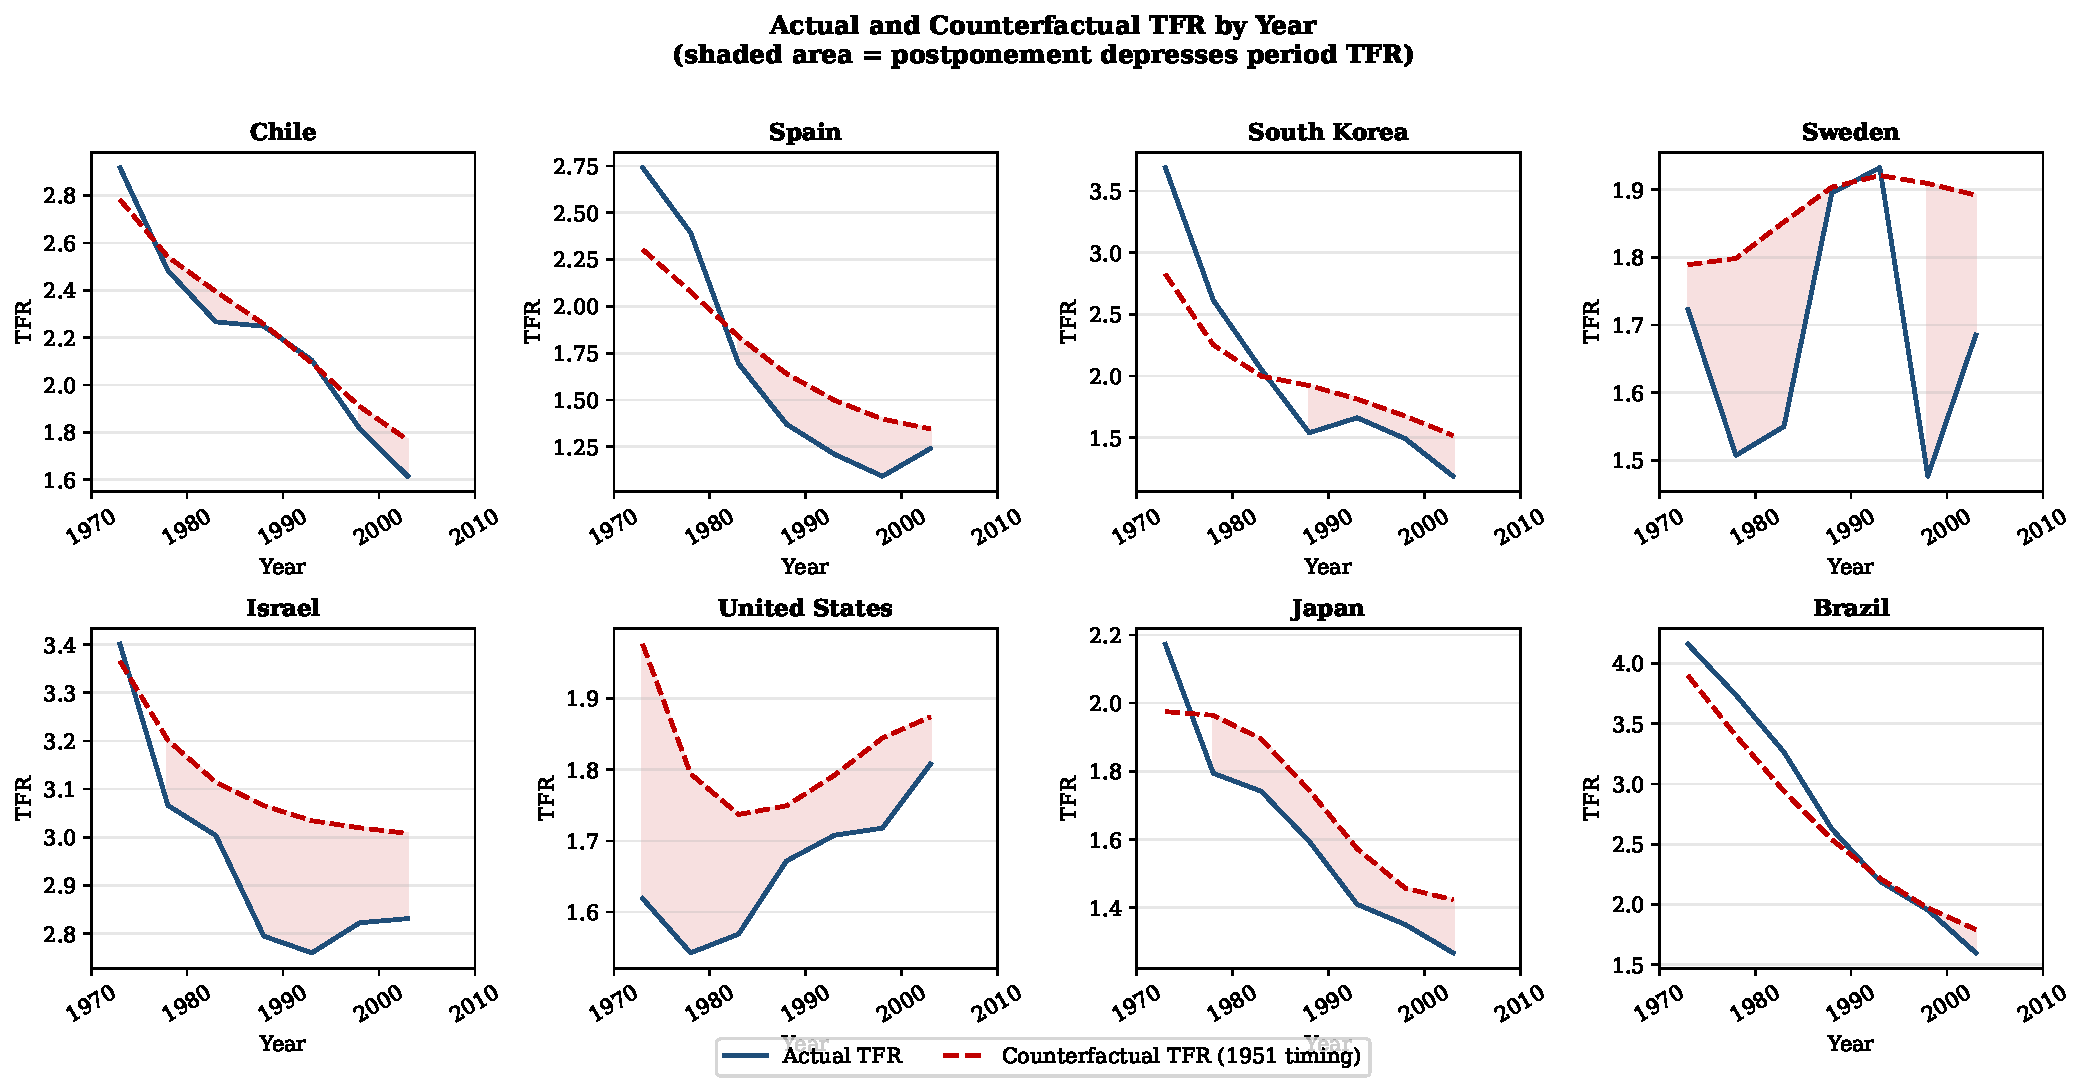
\includegraphics[width=\textwidth]{fig1_actual_vs_cf.pdf}
\caption{Actual Period TFR and Counterfactual TFR for Selected Countries,
         1970--2021. \\
         \emph{Note:} The counterfactual TFR (dashed line) is constructed
         by applying the 1951 birth cohort's age distribution of fertility
         to each subsequent cohort's total quantum.  The vertical gap
         between the two series is the timing (postponement) effect.
         Negative gaps (actual below counterfactual) indicate ongoing
         postponement that depresses period TFR.  Source: authors'
         calculations based on UN WPP / Our World in Data.}
\label{fig:actual_vs_cf}
\end{figure}

\begin{figure}[H]
\centering
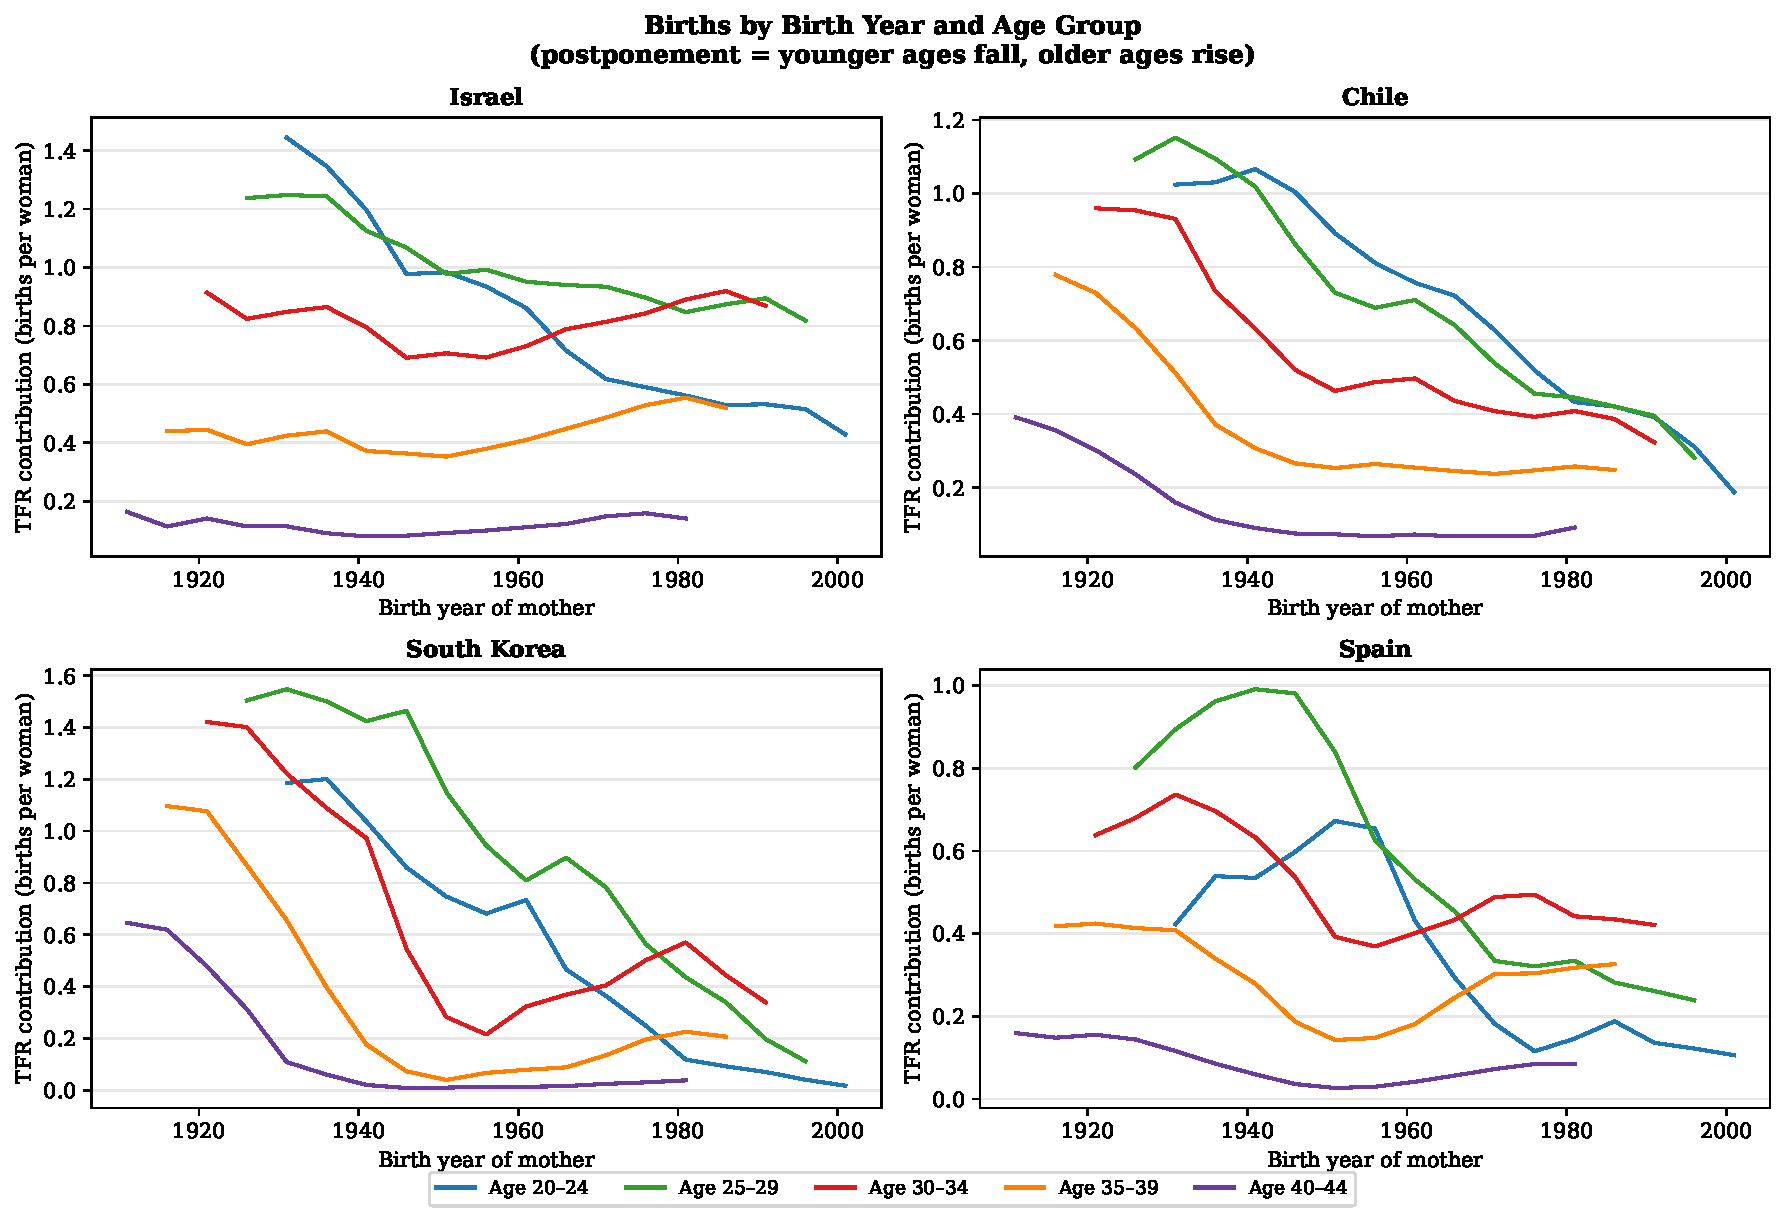
\includegraphics[width=\textwidth]{fig2_cohort_age_profiles.pdf}
\caption{Births by Birth Year and Age Group for Selected Countries. \\
         \emph{Note:} Each line traces the fertility contribution of women in
         a given five-year age group, plotted against the birth year of those
         women.  Rising contributions from older age groups (e.g., 30--34,
         35--39) and falling contributions from younger age groups (20--24,
         25--29) across successive birth cohorts reflect the postponement
         transition.  Source: authors' calculations based on UN WPP / Our
         World in Data.}
\label{fig:cohort_profiles}
\end{figure}

\begin{figure}[H]
\centering
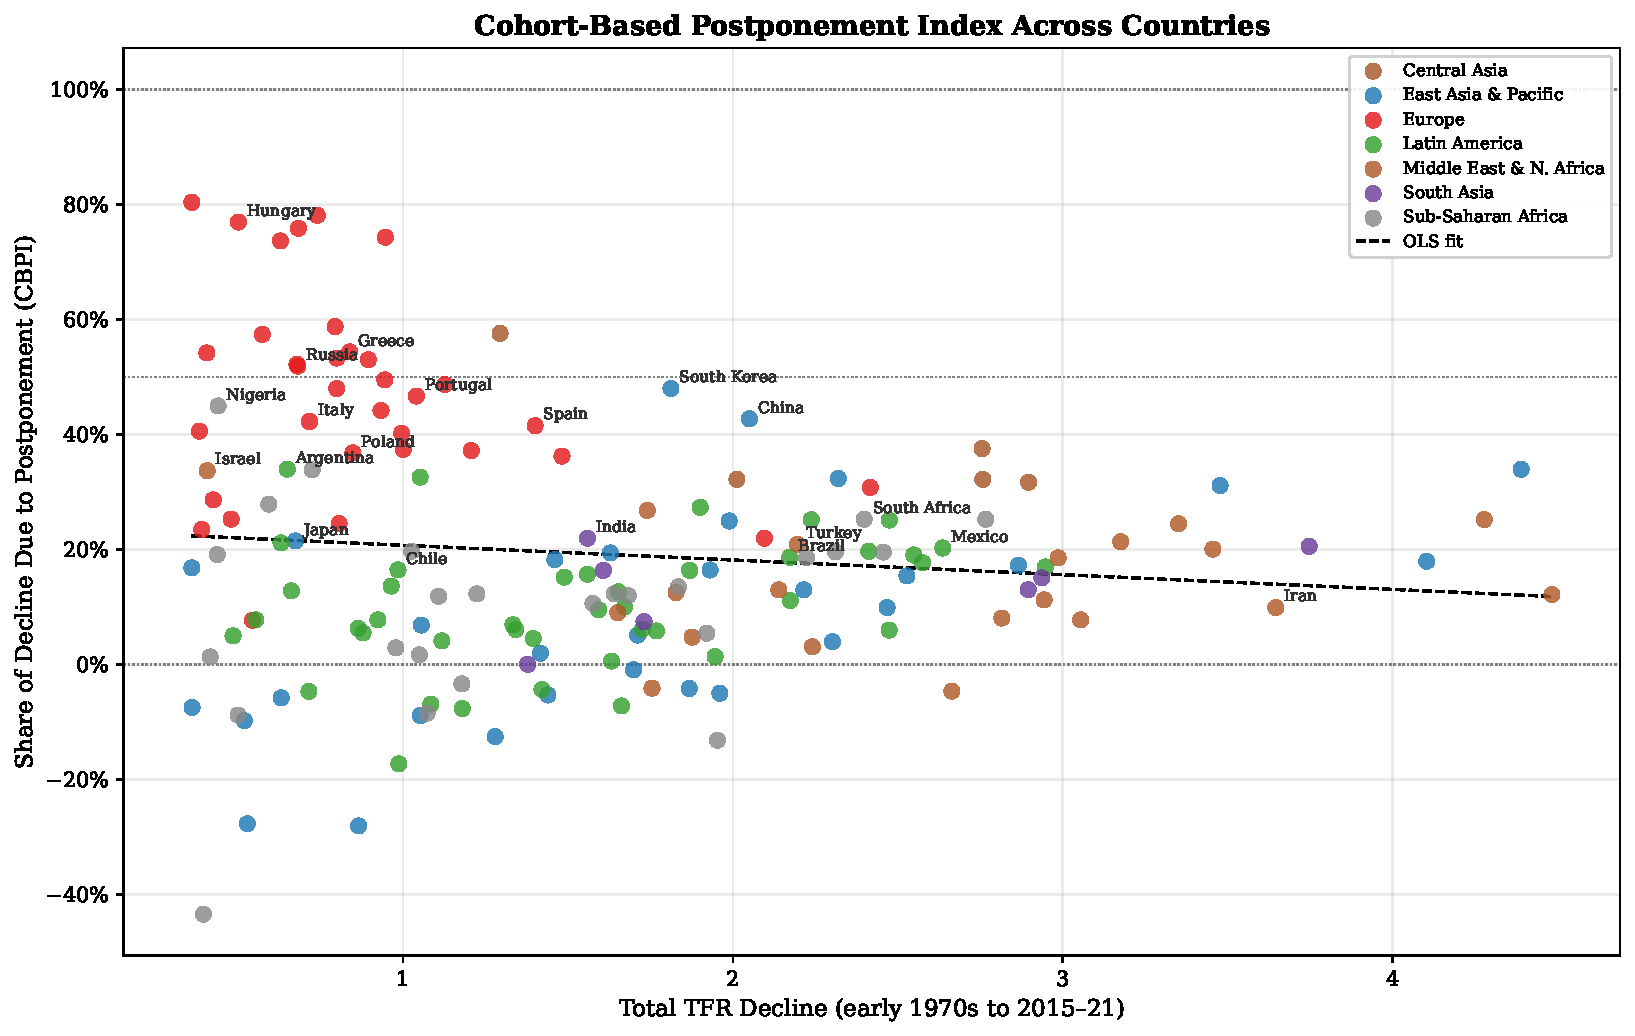
\includegraphics[width=\textwidth]{fig3_postponement_scatter.pdf}
\caption{Cohort-Based Postponement Index (CBPI) Versus Total TFR Decline,
         by Country. \\
         \emph{Note:} Each point represents one country.  The vertical axis
         shows the share of total TFR decline (early 1970s to 2015--21)
         attributable to changes in birth timing (the CBPI).  The horizontal
         axis shows the total observed TFR decline.  Dashed line: OLS fit.
         Source: authors' calculations.}
\label{fig:scatter}
\end{figure}

\begin{figure}[H]
\centering
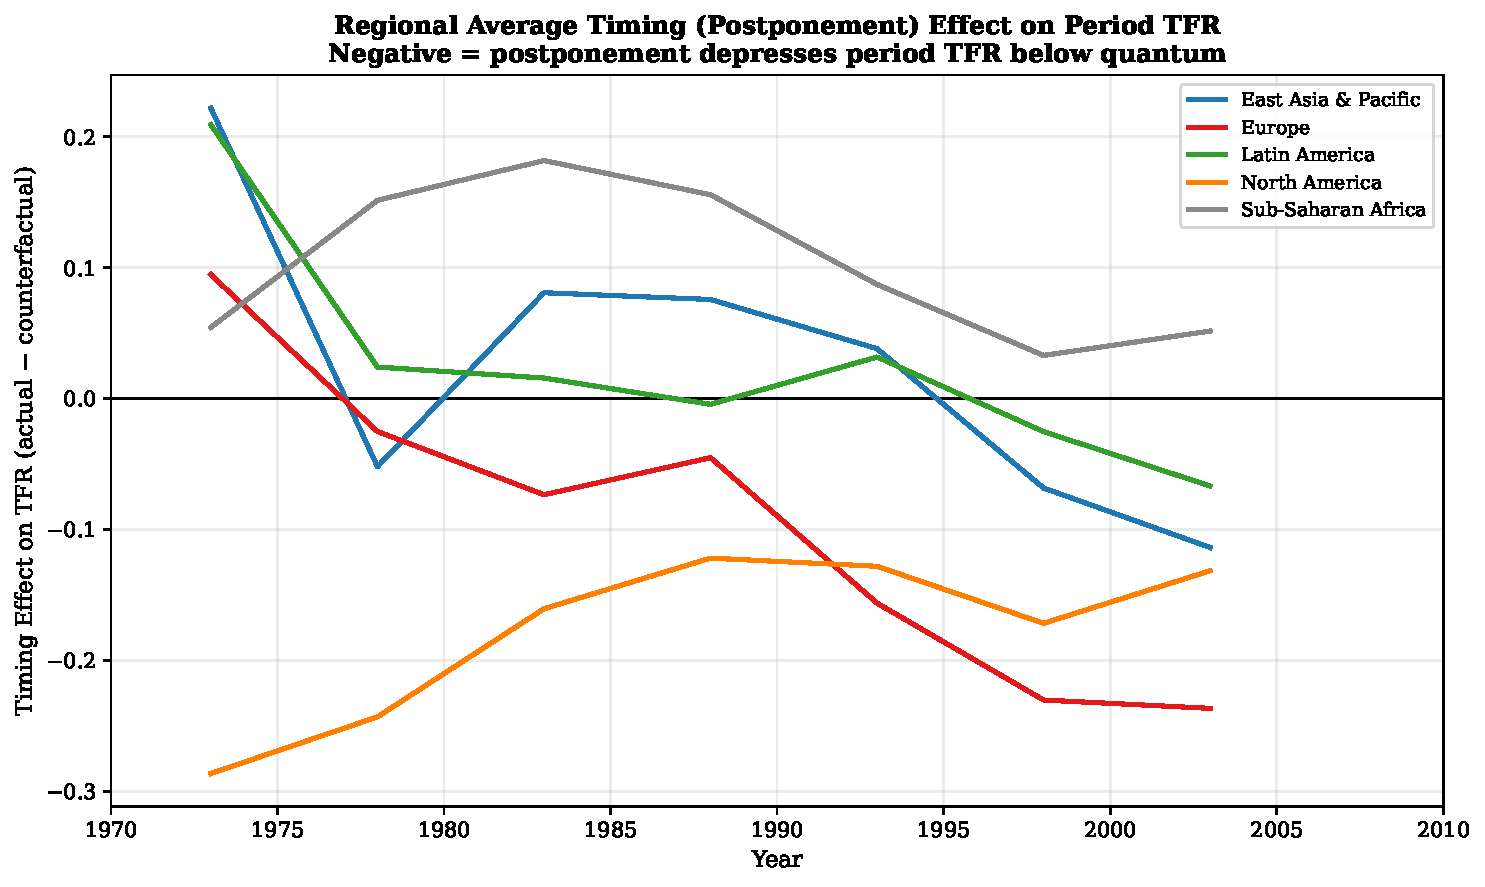
\includegraphics[width=0.9\textwidth]{fig4_timing_effect_regions.pdf}
\caption{Regional Average Timing Effect on Period TFR, 1970--2021. \\
         \emph{Note:} The timing effect is $\mathrm{TE}(t) =
         \mathrm{TFR}(t) - \mathrm{CTFR}(t)$.  Negative values indicate that
         postponement (relative to the 1951 cohort timing) is depressing
         period TFR below the quantum.  Regional averages are unweighted means
         over available countries.  Source: authors' calculations.}
\label{fig:timing_regions}
\end{figure}

\begin{figure}[H]
\centering
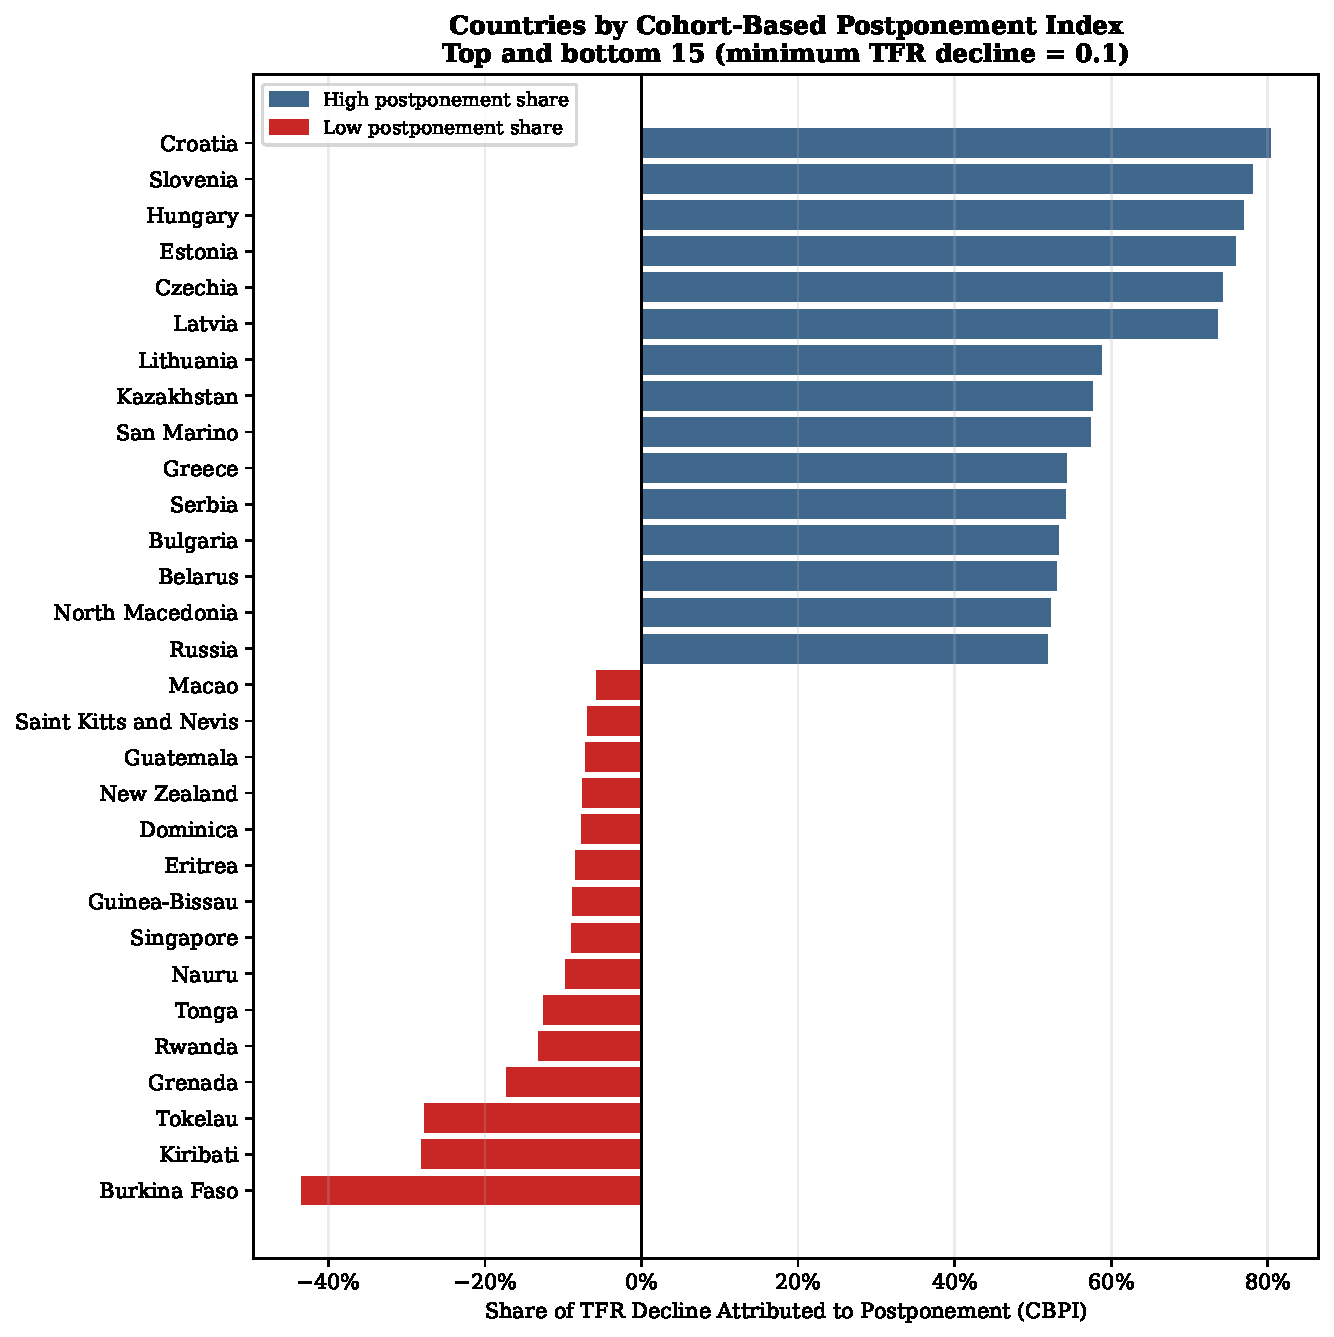
\includegraphics[width=0.9\textwidth]{fig5_postponement_bar.pdf}
\caption{Countries Ranked by Cohort-Based Postponement Index (CBPI). \\
         \emph{Note:} Top and bottom 15 countries by CBPI, restricted to
         countries with a total TFR decline of at least 0.1 TFR points.
         Source: authors' calculations.}
\label{fig:bar}
\end{figure}

% ============================================================
\clearpage
\bibliographystyle{demography}

\begin{thebibliography}{99}

\bibitem[Andersson(2004)]{Andersson2004}
Andersson, G. (2004). Childbearing after migration: Fertility patterns of
foreign-born women in Sweden. \textit{International Migration Review},
38(2), 747--774.

\bibitem[Beaujouan(2019)]{Beaujouan2019}
Beaujouan, E. (2019). Latest-late fertility? Decline and resurgence of late
parenthood across the low-fertility countries. \textit{Population and
Development Review}, 46(2), 219--247.

\bibitem[Blossfeld et al.(2009)]{Blossfeld2009}
Blossfeld, H.-P., Klijzing, E., Mills, M., \& Kurz, K. (Eds.). (2009).
\textit{Globalization, Uncertainty and Youth in Society}. Routledge.

\bibitem[Bongaarts(2009)]{Bongaarts2009}
Bongaarts, J. (2009). Completing the fertility transition in the developing
world: The role of educational differences and fertility preferences.
\textit{Population Studies}, 57(3), 321--335.

\bibitem[Bongaarts \& Feeney(1998)]{BongaartsFeeney1998}
Bongaarts, J., \& Feeney, G. (1998). On the quantum and tempo of fertility.
\textit{Population and Development Review}, 24(2), 271--291.

\bibitem[Bongaarts \& Sobotka(2012)]{BongaartsSobotka2012}
Bongaarts, J., \& Sobotka, T. (2012). A demographic explanation for the
recent rise in European fertility. \textit{Population and Development Review},
38(1), 83--120.

\bibitem[Cavenaghi \& Alves(2011)]{Cavenaghi2011}
Cavenaghi, S., \& Alves, J. E. D. (2011). Diversity of childbearing behavior
within the context of below-replacement fertility in Brazil. In
\textit{International Conference on Population and Development}, Marrakech.

\bibitem[Cohen et al.(2012)]{Cohen2012}
Cohen, A., Dehejia, R., \& Romanov, D. (2012). Financial incentives and
fertility. \textit{Review of Economics and Statistics}, 95(1), 1--20.

\bibitem[Goldscheider et al.(2015)]{Goldscheider2015}
Goldscheider, F., Bernhardt, E., \& Lappeg\aa{}rd, T. (2015). The gender
revolution: A framework for understanding changing family and demographic
behavior. \textit{Population and Development Review}, 41(2), 207--239.

\bibitem[Hoem \& Bramsen(1988)]{HoemBramsen1988}
Hoem, J. M., \& Bramsen, B. (1988). The impact of women's employment on the
transition to parenthood in Sweden. \textit{Stockholm Research Reports in
Demography}, No.\ 49.

\bibitem[Hoem(1993)]{Hoem1993}
Hoem, J. M. (1993). Public policy as the fuel of fertility: Effects of a
policy reform on the pace of childbearing in Sweden in the 1980s.
\textit{Acta Sociologica}, 36(1), 19--31.

\bibitem[Jones \& Gubhaju(2007)]{Jones2007}
Jones, G. W., \& Gubhaju, B. (2007). Trends in age at marriage in the
provinces of Indonesia. \textit{Asian Population Studies}, 5(3), 325--356.

\bibitem[Kim \& Schoen(2000)]{Kim2000}
Kim, Y. J., \& Schoen, R. (2000). On the quantum and tempo of fertility:
Limits to the Bongaarts-Feeney adjustment. \textit{Population and Development
Review}, 26(3), 554--559.

\bibitem[Kohler \& Ortega(2002)]{KohlerOrtega2002}
Kohler, H.-P., \& Ortega, J. A. (2002). Tempo-adjusted period parity
progression measures, fertility postponement and completed cohort fertility.
\textit{Demographic Research}, 6(6), 91--144.

\bibitem[Kohler et al.(2002)]{Kohler2002}
Kohler, H.-P., Billari, F. C., \& Ortega, J. A. (2002). The emergence of
lowest-low fertility in Europe during the 1990s. \textit{Population and
Development Review}, 28(4), 641--680.

\bibitem[Kohler et al.(2002b)]{Kohler2002b}
Kohler, H.-P., Billari, F. C., \& Ortega, J. A. (2002). Low and lowest-low
fertility in Europe: Causes, implications and policy options. In F.\ Raines
(Ed.), \textit{The New Demographic Regime}. UNECE.

\bibitem[Lesthaeghe \& van de Kaa(2002)]{LesthaegheVan2002}
Lesthaeghe, R., \& van de Kaa, D. (2002). Two demographic transitions? In
D. van de Kaa \& R. Lesthaeghe (Eds.), \textit{Bevolking: Groei en Krimp}.
Van Loghum Slaterus, Deventer.

\bibitem[Lesthaeghe(2004)]{Lesthaeghe2004}
Lesthaeghe, R. (2004). The unfolding story of the second demographic
transition. \textit{Population and Development Review}, 36(2), 211--251.

\bibitem[Mills et al.(2011)]{Mills2011}
Mills, M., Rindfuss, R. R., McDonald, P., \& te Velde, E. (2011). Why do
people postpone parenthood? Reasons and social policy incentives.
\textit{Human Reproduction Update}, 17(6), 848--860.

\bibitem[Myrskyl{\"a} et al.(2013)]{Myrskyla2013}
Myrskyl{\"a}, M., Kohler, H.-P., \& Billari, F. C. (2013). New cohort
fertility forecasts for the developed world. \textit{Population and
Development Review}, 39(1), 31--56.

\bibitem[Our World in Data(2024)]{OWID2024}
Our World in Data. (2024). \textit{Fertility Rate by Age Group}. Based on
UN World Population Prospects 2022 revision. Retrieved from
\url{https://ourworldindata.org/fertility-rate}.

\bibitem[Raymo et al.(2015)]{Raymo2015}
Raymo, J. M., Park, H., Xie, Y., \& Yeung, W. J. J. (2015). Marriage and
family in East Asia: Continuity and change. \textit{Annual Review of
Sociology}, 41, 471--492.

\bibitem[Ryder(1964)]{Ryder1964}
Ryder, N. B. (1964). The process of demographic translation.
\textit{Demography}, 1(1), 74--82.

\bibitem[Schoen(2004)]{Schoen2004}
Schoen, R. (2004). Timing effects and the interpretation of period fertility.
\textit{Demography}, 41(4), 801--819.

\bibitem[Sobotka(2003)]{Sobotka2003}
Sobotka, T. (2003). Tempo-quantum and period-cohort interplay in fertility
changes in Austria, the Czech Republic, Hungary, and Slovakia.
\textit{Demographic Research}, 8(6), 151--214.

\bibitem[Sobotka(2004)]{Sobotka2004}
Sobotka, T. (2004). \textit{Postponement of Childbearing and Low Fertility in
Europe}. Dutch University Press, Amsterdam.

\bibitem[Sobotka(2011)]{Sobotka2011}
Sobotka, T. (2011). Fertility in Central and Eastern Europe after 1989: Collapse
and gradual recovery. \textit{Historical Social Research}, 36(2), 246--296.

\bibitem[Sobotka(2017)]{Sobotka2017}
Sobotka, T. (2017). Postponement of childbearing and low fertility in Europe.
In R. Rindfuss \& M. Choe (Eds.), \textit{Low and Lower Fertility}. Springer.

\bibitem[United Nations(2022)]{UNWPP2022}
United Nations, Department of Economic and Social Affairs, Population Division.
(2022). \textit{World Population Prospects 2022}. United Nations.

\bibitem[van Imhoff(2001)]{vanImhoff2001}
van Imhoff, E. (2001). On the impossibility of inferring cohort fertility
measures from period fertility measures. \textit{Demographic Research},
5(2), 23--64.

\bibitem[Westoff(2011)]{Westoff2011}
Westoff, C. F. (2011). \textit{Desired Number of Children: 2000--2008}.
DHS Comparative Reports, No.\ 25. ICF Macro.

\bibitem[World Bank(2023)]{WorldBank2023}
World Bank. (2023). \textit{World Development Indicators}. Washington, DC:
The World Bank Group.

\bibitem[Zeng \& Land(2011)]{Zeng2011}
Zeng, Y., \& Land, K. C. (2011). Adjusting period tempo changes with an
extension of Ryder's basic translation equation. \textit{Demography},
38(2), 317--328.

\end{thebibliography}

\end{document}
